\section{State of the art\label{chap:state_of_the_art}}
\ajax{} is a widely used technique in the internet to build web applications because of the user experience improvements it features.
In \cite{roodt2006effect} is mentioned that \ajax{} applications have a better usability than non-\ajax{} \webSite{}s.
The same conclusion is made in \cite{kluge2007effects}, despite the lack of browser navigation support.
Besides the navigation problem, another disadvantage is, as presented in \cite{mesbah2009analysis}, crawling \ajax{} applications is not trivial.
One solution to this task is finding clickables and navigating to every page found.
Nevertheless \cite{mesbah2009analysis} also states that this only generates a snapshot of the full application.
Even search engines are avoiding to crawl \webSite{}s because of it's difficulty\cite{duda2009ajax}.
Currently the task of building a crawlable \singlePageApplication{} using \ajax{} is often avoided. Instead crawling algorithms are improved and in focus of research. One example for this is  like \emph{ATUSO} \cite{mesbah2012invariant}.

\subsection{Client-side rendering\label{sec:state_client_side_rendering}}
When building an asynchronous web application it is possible to render the pages in the client or in the server.
A lot of \ajax{} applications use a JSON API which already predefines the outcome of this decision:
\\
JSON is sent by the server, interpreted and rendered by the \ajax{}-engine in the client.
An advantage of this practice is the strong separation of the logic on the server and views on the client-side.
This \webApplication{} design also reduces the server load as the computation of rendering the data is made in the client.
The overhead of HTML markup for styles and the UI is not sent for every \webPage{} anymore which additionally reduces the traffic.
As plain string modifications are difficult to maintain especially on large applications, client-side templates become more and more widespread.
\\
As the web server does not render \webPage{}s, it is hard to create snapshots for search engines.
Headless browsers like Phantom.js\footnote{\url{http://phantomjs.org/} (Accessed: Juli 28, 2015)} can render such pages and serve them for crawlers.
\\
Figure \ref{fig:frontend_snapshots} shows the flow of a request by a crawler with the use of a headless browser and HashBang URLs, introcuded in \ref{hashbangurls}.
After the initial crawl request is made, the web server lets the server-side headless browser render a snapshot of the HTML and then response to the crawler with this snapshot.

\begin{figure}[H]
\centering
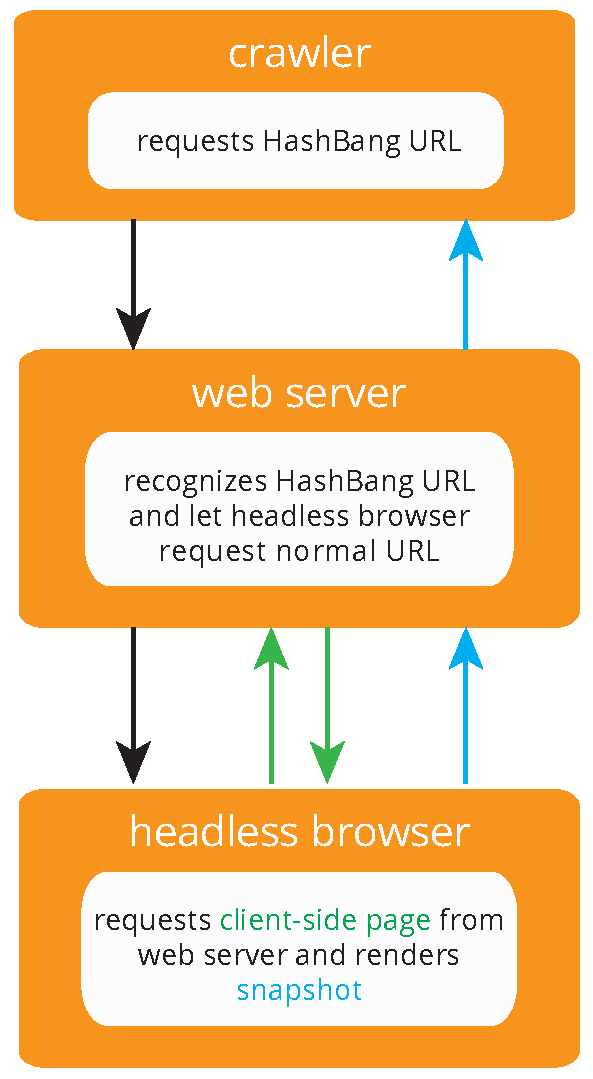
\includegraphics[height=10cm]{images/frontend_snapshots.pdf}
\caption[frontend_snapshots]{Rendering client-side rendered pages with headless browser}
\label{fig:frontend_snapshots}
\end{figure}

\subsubsection{Load time analysis}
With client-side rendering at least three requests are needed, before data is rendered:
\begin{enumerate}
    \item An HTML file containing a link to the \ajax{} engine and frontend templates.
    \item The \ajax{} engine itself.
    \item Data which should be rendered into the templates.
\end{enumerate}

\noindent{}It is not possible to run the three requests listed above in any other order or concurrently, because the \ajax{} engine is linked in the initial HTML file and the data gets requested by the \ajax{} engine.
\\
Sometimes the frontend templates must be requested additionally if they are not part of the HTML document or the AJAX engine.
Those template requests could be made concurrently to retriev the data, which is the reason that those further requests are ignored in the following analysis.
\\
To get a bit more into detail this means a series of requests and responses.
Mike Belshe states in \cite{belshe2010more} \enquote{More bandwidth doesn't matter (much)}.
Considering this and the fact he states that Round Trip Times influence the Web in a bigger way than bandwidth, we neglect data transfer in the following analysis.
\\
As HTTP is based on TCP it first has to make a handshake, which takes one RTT.
All of those three requests take at least one additional RTT, too.
This means it is necessary to wait at least four RTTs before the page starts to be rendered.
Taking the RTT of 70ms, used in \cite{spero1994analysis}, this means a waiting time of 280ms before rendering can start.
\\
An efficient \webApplication{} which uses client-side rendering requests one URL on which the response contains all needed data.
If more requests are needed an additional RTT per request has to be added to the example above.
\\
Despite the fact that the server could need additional time to render the page, common \httpRequest{}s need 2 RTTs less than this pattern.

\subsection{\ClientSideMVC{}\label{sec:state_client_side_mvc}}
In addition to only outsource the templating to the frontend, there are complete client-side MVC frameworks.
Those frameworks use the model view controller pattern, where the controller has a connection to the web server.
\\
Built on REST APIs\footnote{\url{http://www.peej.co.uk/articles/rest.html} (Accessed: Juli 28, 2015)} they move all logic into the client-side.
This approach is built primarily on the motivation to reduce the web server load and traffic.
\\
The initial request is divided into the three requests as shown in section \ref{sec:state_client_side_rendering}.
Further requests are not made to request URLs in the old fashioned way, but to retrieve objects through a REST API. 
Object manipulation, logical methods and everything normally implemented in a server backend should be in the frontend in those frameworks.
\\
Using this pattern, the same problems as with client-side templates will appear but on another level.
Instead of the web server, the client decides which information it needs and requests it from the server and renders those.
\\
Load and traffic of the server in this pattern is relatively low, because it will only create, update, delete or retrieve objects in the database. 
More logical functions on the server-side are not needed normally.
\\
Clients, especially mobile devices and slow computers, might struggle with the load of work instead.
\\
The most used client-side MVC framework is AngularJS\footnote{\url{https://angularjs.org/} (Accessed: Juli 28, 2015)}. In the evaluation in chapter \ref{chap:evaluation} it also represents this kind of \webApplication{}s.

\subsubsection{Load time analysis}
Similar to simple client-side templates mentioned in \ref{sec:state_client_side_rendering}, client-side MVCs need at least three requests to render the first page.
In most cases more than one model needs to be known by the client to render a page, which increases the amount of requests to render a page.
\\
To get into more detail, the client needs to wait for the first request to be completed, then the \ajax{} engine has to be loaded.
After the initialization of the \ajax{} engine, it requests the needed data.
\\
We are using 70ms as RTT as stated in \ref{sec:state_client_side_rendering} and get a result of 280ms for those three requests.
This result is the optimal result which can be achieved, but often it is much higher, because there is not one but multiple objects which have to be fetched independently.
It is not always possible to request all data concurrently, e.g. when a second object is linked in a first one.
In this case the first object has to be fetched and afterwards the second one if it's not known or linked before.

\subsection{Hash-Bang URLs\label{hashbangurls}}
In order to have a working SEO in SPAs it is recommended by Google to use hashbang URLs.
This pattern defines that in the URL the \emph{hash part} should start with \enquote{\#!} instead of only \enquote{\#}.
Finding this combination let crawlers know that the site provides an AJAX application and additionally full page snapshots created using techniques like shown in \ref{sec:state_client_side_rendering}.
When a crawler e.g. finds an URL like \url{http://example.com/\#!site=test1} it crawls \newline \url{http://example.com/?\_escaped\_fragment\_=site=test1} instead.
This is done, because everything after the \enquote{\#} will not be sent to the server, but is only recognized by the client.
To let the server know that a specific page should be requested this URL modification is needed.
At this \enquote{?\_escaped\_fragment\_=} URL a snapshot of the full page should be available.
This means, instead of only providing a few parts of the page required by \ajax{}, the whole HTML DOM should be delivered.
\\
On the other hand the \ajax{} engine can recognize everything behind the \enquote{\#} and requests the data needed for the page, lead to by the ongoing part.
\\
This technique was developed for URL changing by JavaScript without a full page reload.
Old browsers without the implementation of the History API are not able to change the URL without a full load of a page.
To gain navigation functionality on \singlePageApplication{}s the only way was to change the hash value in the URL, which does not call a page load, but updates the URL and pushes it to the navigation history.

\subsection{\hijax{}\label{hijax}}
Another way to implement \singlePageApplication{}s using \ajax{} is to use the development pattern of HIJAX.
When using PJAX and \lare{}, introduced in section \ref{sec:state_pjax} and chapter \ref{chap:lare}, the usage of this pattern is recommended.
\\
When developing a \webSite{} using this pattern, it should be planned with the use of \ajax{} but in the first step implemented serving just common \httpRequest{}s.
Changes of the HTML markup in favour of \ajax{} should be avoided at this step.
Every \webPage{} should be delivered fully and links should be linking to real \webPage{}s.
No JavaScript should be needed to link \webPage{}s within the site.
\\
After the \webSite{} is implemented completely the event listeners on the links can be \emph{hijacked} and processed by JavaScript.
A good way to do that is using classes in the linking tag which gain semantics in JavaScript.
This script then creates a new XMLHttpRequest which requests only the updated parts of the page and renders the response.
\\
When this pattern is used the \webSite{} degrades gracefully.
This means even when JavaScript is not available or blocked, the \webSite{} still works, a client can still discover the single pages and a crawler sees the whole content.

\subsection{PJAX\label{sec:state_pjax}}
PJAX, introduced 2011 by Chris Wanstrath, \enquote{is a jQuery plugin that uses AJAX and pushState to deliver a fast browsing experience with real permalinks, page titles, and a working back button.}\footnote{\url{https://github.com/defunkt/jquery-pjax\#introduction} (Accessed: Juli 28, 2015)}
Using it makes it possible to use the HIJAX pattern, introduced in \ref{hijax}.
\\
PJAX let the browser replace a container in a page by requesting a URL in a certain way like adding a \enquote{?pjax} query parameter.
When requesting a page like e.g. \url{http://example.com/test/} a full page is responded.
Requests at \url{http://example.com/test/?pjax} will be responded with only one container.
In combination with \hijax{} it is possible to have anchor tags like \emph{<a href="/test/" class="pjax">\newline{}test</a>} while PJAX requests \url{http://example.com/test/?pjax}.
\\
Crawlers which are not able to interpret JavaScript crawl all pages in the common way.
Browsers which are able to interpret JavaScript instead will have the advantages of AJAX.
\\
PJAX has the ability to either send one specific container or a full page per URL. 
Without great effort it is not able to send containers according to the client's previous page.
